% (c) 2012-2013 Claudio Carboncini - claudio.carboncini@gmail.com
% (c) 2012-2014 Dimitrios Vrettos - d.vrettos@gmail.com
% (c) 2015 Daniele Zambelli daniele.zambelli@gmail.com

\chapter{Trigonometria}

 
\section{Prime definizioni}
\label{sec:trigo_primedef}

L'etimologia della parola ``trigonometria'' dal greco \emph{trígonon} 
(triangolo) e \emph{métron} (misura) chiarisce in cosa consiste
questa parte della matematica che ci accingiamo ad affrontare.
La \emph{trigonometria} nasce dal problema di \emph{risolvere un triangolo}, 
cioè di ricavare la misura di alcuni suoi elementi incogniti date
le misure di altri elementi. Dal momento che gli elementi di un triangolo sono 
sei, i tre lati e i tre angoli, vedremo come, date le misure di
almeno tre di questi elementi di cui almeno uno sia un lato, sia possibile 
determinare la misura degli altri tre elementi mancanti.

\begin{multicols}{2}
 Disegniamo un triangolo rettangolo, retto in~$A$, avendo cura di indicare con 
la stessa lettera vertice e lato opposto, come nella figura a fianco.
Ricordiamo che tra i lati sussiste la relazione del teorema di 
Pitagora~$\overline{BC}^{2}=\overline{AC}^{2}+\overline{AB}^{2}$ e che ciascun 
cateto
è minore dell'ipotenusa. Ricordiamo anche che gli angoli acuti sono 
complementari~$\widehat {C}+\widehat {B}=90\grado$.
\begin{center}
\begin{inaccessibleblock}[Triangolo rettangolo, 
l'angolo di vertice A ($\alpha$) è retto il lato opposto si chiama ``a'';
l'angolo di vertice B si chiama $\beta$, il lato opposto si chiama ``b'';
l'angolo di vertice C si chiama $\gamma$, il lato opposto si chiama ``c''.]
 % (c) 2012 Dimitrios Vrettos - d.vrettos@gmail.com
% (c) 2020 Daniele Zambelli: daniele.zambelli@gmail.com

% \tkzMarkAngles(C,B,M B,M,C M,C,B%
% D,L,N L,N,D N,D,L)
% \tkzFillAngles[fill=red!20,opacity=.2](C,B,M%
% B,M,C M,C,B D,L,N L,N,D N,D,L)

\begin{tikzpicture}[x=10mm,y=10mm, font=\small]

\coordinate (A) at (0,0);
\coordinate (B) at ($(A)+(0:4)$);
\coordinate (C) at ($(A)+(90:2.5)$);

\draw (A) node[below left]  {$A$} -- 
      (B) node[below right] {$B$} node[midway,below]{$c$} -- 
      (C) node[above left]  {$C$} node[midway,above]{$a$} --
      (A)                         node[midway,left] {$b$};

\tkzFillAngles[fill=LimeGreen, draw, size=.33](A,C,B C,B,A)
\tkzLabelAngle[pos=.6](A,C,B){$\gamma$}

% \tkzFillAngle[fill=LimeGreen, draw, size=.33](C,B,A)
\tkzLabelAngle[pos=.6](C,B,A){$\beta$}

\tkzMarkRightAngle[fill=LimeGreen, draw, size=.2](C,A,B);
\tkzLabelAngle[pos=.4](B,A,C){$\alpha$}

\end{tikzpicture}

\end{inaccessibleblock}
\end{center}
\end{multicols}

\osservazione Basta conoscere la misura di due lati per determinare la misura 
del terzo lato, ma queste informazioni non ci permettono di determinare
l'ampiezza degli angoli acuti se non in casi particolari. Se conosciamo un 
angolo acuto e la misura di un lato non possiamo determinare la misura
degli altri elementi mancanti.

Riferendoci alla figura, chiamiamo cateto adiacente all'angolo 
acuto~$\hat{\beta}$ il cateto~${AB}$ indicato con~$c$ e cateto opposto 
all'angolo~$\hat{\beta}$ il
cateto~${AC}$ indicato con~$b$.

\begin{definizione}
Seno, coseno, tangente
\begin{align*}
&\sin \beta=\frac{\text{cateto opposto}}{\text{ipotenusa}}=
\frac{AC}{CB}=\frac{b}{a} \quad \Rightarrow \quad b=a\cdot \sin \beta ;\\
&\cos \beta=\frac{\text{cateto adiacente}}{\text{ipotenusa}}=
\frac{AB}{CB}=\frac{c}{a} \quad \Rightarrow \quad c=a\cdot \cos \beta ;\\
&\tan \beta=\frac{\text{cateto opposto}}{\text{cateto adiacente}}=
\frac{AC}{AB}=\frac{b}{c} \quad \Rightarrow \quad b=c\cdot \tan(\beta ).
\end{align*}
\end{definizione}

% \newpage

% \begin{definizione}
% Per l'angolo~$\hat{\gamma} =90\grado -\hat{\beta}$ complementare 
% di~$\hat{\beta}$:
% \begin{align*}
%  &\sin \gamma=\frac{\text{cateto 
% opposto}}{\text{ipotenusa}}=\frac{AB}{CB}=\frac{c}{a}\text{, da cui }c=a\cdot 
% \sin \gamma ;\\
% &\cos \gamma=\frac{\text{cateto 
% adiacente}}{\text{ipotenusa}}=\frac{AC}{CB}=\frac{b}{a}\text{, da cui }b=a\cdot 
% \cos \gamma ;\\
% &\tan \gamma=\frac{\text{cateto opposto}}{\text{cateto 
% adiacente}}=\frac{AB}{AC}=\frac{c}{b}\text{, da cui }c=b\cdot \tan(\gamma ).
% \end{align*}
% \end{definizione}

Le definizioni sono ben poste: le funzioni \emph{seno dell'angolo} (sen 
o~$\sin$), \emph{coseno dell'angolo} ($\cos$), \emph{tangente dell'angolo}
($\tan$ o tg) dipendono solo dagli angoli e non dal particolare triangolo usato. 
Infatti angoli acuti della stessa misura appartengono a
triangoli rettangoli tutti simili tra loro; siccome i lati di triangoli simili 
sono in proporzione, il rapporto tra i lati è invariato.
Inoltre possiamo certamente affermare che le funzioni seno e coseno di angoli 
acuti assumono valori positivi minori di~$1$,
poiché in un triangolo rettangolo il cateto è minore dell'ipotenusa.

Dal confronto delle definizioni notiamo che valgono le uguaglianze:
 \[\sin \gamma=\cos \beta;\quad \cos \gamma=\sin \beta;\quad \tan 
\gamma=\frac{1}{\tan \beta},\]
 per cui possiamo anche scrivere:
\[\sin x=\cos (90\grado-x);\quad \cos x=\sin (90\grado-x);\quad 
\tan x=\frac{1}{\tan(90\grado-x)}.\]

\begin{exrig}
 \begin{esempio}
Nel triangolo rettangolo~$ABC$ i cateti misurano rispettivamente~$AB=4\unit{m}$, 
$AC=3\unit{m}$ e l'ipotenusa misura~$5\unit{m}$.
Possiamo determinare le funzioni goniometriche dei suoi angoli acuti 
semplicemente applicando le definizioni.
Si ottiene
\[\sin \beta =\frac{b}{a}=\frac{3}{5};\quad \cos (\beta 
)=\frac{c}{a}=\frac{4}{5};\quad \tan (\beta )=\frac{b}{c}=\frac{3}{4}.\]
Per l'angolo complementare lasciamo al lettore il completamento:
$\sin \gamma =\ldots\ldots$\quad~$\cos \gamma =\ldots\ldots$\quad~$\tan(\gamma 
)=\ldots\ldots$\quad.
 \end{esempio}
\end{exrig}

\osservazione Ancora non possiamo avere informazioni sull'ampiezza degli angoli 
acuti;
vedremo in seguito come procedere nei calcoli e quindi concludere la risoluzione 
del triangolo.

% \vspace{1.10ex}
% \ovalbox{\risolvi \ref{ese:G.1}}

\section{Due identità fondamentali}
\label{sec:trigo_identita}

Dalle definizioni date nella sezione precedente abbiamo queste due identità 
fondamentali:
\[\tan \gamma=\frac{a\cdot \sin \gamma}{a\cdot \cos \gamma}=
\frac{\sin \gamma}{\cos \gamma}.\]
La tangente di un angolo è il rapporto tra il seno dell'angolo e il coseno dello 
stesso angolo. In generale:
 \begin{equation}
 \tan x=\frac{\sin x}{\cos x}.
 \end{equation}

Dal teorema di Pitagora si ha~$a^{2}=b^{2}+c^{2}$ da cui dividendo ambo i membri 
per~$a^{2}$ si ottiene
\begin{align*}
&\frac{a^{2}}{a^{2}}=\frac{b^{2}+c^{2}}{a^{2}}=
\frac{b^{2}}{a^{2}}+\frac{c^{2}}{a^{2}}\\
\Rightarrow & 1=\left(\frac{b}{a}\right)^{2}+\left(\frac{c}{a}\right)^{2}\\
\Rightarrow & 1=\left(\cos \gamma\right)^{2}+\left(\cos  \gamma\right)^{2}\\
\Rightarrow & 1=\cos^{2} \gamma+\sin^{2} \gamma.
\end{align*}
In generale, per qualunque angolo~$x$ vale
\begin{equation}
\label{eq:F.2}
 \cos^{2}(x)+\sin^{2}(x)=1.
\end{equation}
Si definiscono inoltre altre funzioni goniometriche che potranno servire nella 
risoluzione dei triangoli:
$\csc(x)=\frac{1}{\sin x}$\quad~$\sec(x)=\frac{1}{\cos x}$\quad~$\cot(x)=
\frac{1}{\tan x}$.

\begin{exrig}
 \begin{esempio}
In un triangolo rettangolo si sa che~$\cos \beta=\frac{3}{4}$, 
determinare~$\sin \beta$ e~$\tan \beta$.

\emph{Strategia risolutiva:}
ricordando che per qualunque angolo~$x$ vale la~\ref{eq:F.2} possiamo sostituire 
il dato e calcolare
$\sin \beta=\sqrt{1-\cos ^{2}(\beta 
)}=\sqrt{1-\frac{9}{16}}=\frac{\sqrt{7}}{4}$. 
Infine sapendo che per ogni angolo vale~$\tan x=\frac{\sin x}{\cos (x)}$ 
ricaviamo:
\[\tan \beta=\cfrac{\cfrac{\sqrt{7}}{4}}{\cfrac{3}{4}}=\frac{\sqrt{7}}{3}.\]
Osserviamo che nella determinazione di~$\sin \beta$ abbiamo trascurato il valore 
negativo in quanto abbiamo definito
le funzioni goniometriche come rapporto delle misure di due segmenti.
 \end{esempio}
\end{exrig}

\ovalbox{\risolvi \ref{ese:G.2}}

\section{Angoli particolari}
\label{sec:trigo_angoliparticolari}
Possiamo ricavare per via geometrica il valore esatto delle funzioni 
goniometriche di angoli particolari.

\subsection{Angoli di~45°}

 Il triangolo rettangolo isoscele (figura~\ref{fig:G.1}) i cui angoli acuti sono 
di~$45\grado$ è la metà di un quadrato di lato~$1$.
Sappiamo che~$d=\sqrt{1^{2}+1^{2}}=\sqrt{2}$ poiché il calcolo delle funzioni 
goniometriche per un angolo
non dipende dal particolare triangolo usato, possiamo concludere per le 
definizioni date:
$\sin 45\grado=\frac{1}{\sqrt{2}}=\frac{\sqrt{2}}{2}$ e anche
$\cos (45\grado)=\frac{\sqrt{2}}{2}$ e per la definizione di tangente 
dell'angolo~$\tan (45\grado)=1$.%[figura~3]

\begin{inaccessibleblock}[Triangolo rettangolo isoscele e 
triangolo equilatero diviso dall'altezza in due triangoli rettangoli 30-60]
 \begin{figure}[t]
\begin{minipage}[t]{.45\textwidth}
 \centering
 % (c) 2012 Dimitrios Vrettos - d.vrettos@gmail.com

\begin{tikzpicture}[x=10mm,y=10mm, font=\small]

\coordinate (B) at (0,0);
\coordinate (A) at ($(B)+(0:-2.5)$);
\coordinate (C) at ($(B)+(90:2.5)$);
\draw (A) node[below left]{$A$} -- (B) node[below right]{$B$}node[midway,below]{$l$} -- (C)node[above right]{$C$} -- (A)node[midway,left]{$d$};

\node[above left]at (-2.5,2.5) {$D$};
\tkzMarkAngle[ fill=LimeGreen ,draw, size=.3](B,A,C)

\tkzLabelAngle[below, pos=1](C,A,B){$\alpha=45\grado$}
\begin{scope}[fill=CornflowerBlue, draw=black]
\filldraw (0,0) circle (1pt);
\filldraw (0,2.5) circle (1pt);
\filldraw (-2.5,0) circle (1pt);
\filldraw (-2.5,2.5) circle (1pt);
\end{scope}

\begin{scope}[dotted]
\draw (-2.5,0) -- (-2.5,2.5)-- (0,2.5);
\end{scope}

\end{tikzpicture}
 \caption{Triangolo rettangolo isoscele.}\label{fig:G.1}
\end{minipage}\hfil
\begin{minipage}[t]{.45\textwidth}
 \centering
 % (c) 2012 Dimitrios Vrettos - d.vrettos@gmail.com

\begin{tikzpicture}[x=10mm,y=10mm, font=\small]
  \coordinate (H) at (0,0);
  \coordinate (A) at ($(H)+(90:2.6)$);
  \coordinate (C) at ($(H)+(0:1.3)$);
  \coordinate (B) at ($(H)+(0:-1.3)$);
  \draw (A) node[above]{$A$} -- (B) node[below left]{$B$} -- (H)node[below]{$H$}  -- (A)-- (C)node[below right]{$C$} -- (H);

  \tkzMarkAngle[ fill=LimeGreen ,draw, size=.4](H,A,C)
  \tkzMarkAngle[ fill=LimeGreen ,draw, size=.3](A,C,H)
  \tkzMarkRightAngle[fill=LimeGreen,draw, size=.2](A,H,C)
  
  \begin{scope}[font=\scriptsize]
    \tkzLabelAngle[pos=.9](C,A,H){$30\grado$}
    \tkzLabelAngle[pos=.5](H,C,A){$60\grado$}
    \tkzLabelAngle[pos=.5](A,H,C){$90\grado$}
  \end{scope}

  \begin{scope}[fill=CornflowerBlue, draw=black]
    \filldraw (0,0) circle (1pt);
    \filldraw (0,2.6) circle (1pt);
    \filldraw (-1.3,0) circle (1pt);
    \filldraw (1.3,0) circle (1pt);
  \end{scope}

\end{tikzpicture}
 \caption{Triangolo rettangolo con angoli di~$30\grado$ 
e~$60\grado$.}\label{fig:G.2}
\end{minipage}
\end{figure}
\end{inaccessibleblock}

\subsection{Angoli di~30° e~60°}
Il triangolo rettangolo con un angolo di~$30\grado$ ha l'altro angolo acuto 
di~$60\grado$ (figura~\ref{fig:G.2}) pertanto possiamo trattare insieme
la ricerca delle funzioni goniometriche di tali angoli.

Il triangolo rettangolo in questione è la metà di un triangolo equilatero di 
lato~$1$ e altezza~$h$ poiché $\overline{HC}$ è metà del lato
possiamo subito dire che~$\cos 60\grado=\frac{\overline{HC}}{1}=\frac{1}{2}$.
Per le definizioni date si ha~$\sin 60\grado=\frac{\overline{AH}}{1}$.
Applicando il teorema di Pitagora si ottiene
\[\overline{AH}=\sqrt{1^{2}-\left(\frac{1}{2}\right)^{2}}=\sqrt{1-\frac{1}{4}}=
\sqrt{\frac{3}{4}}=\frac{\sqrt{3}}{\sqrt{4}}=\frac{\sqrt{3}}{2}
\Rightarrow\sin 60\grado=\frac{\sqrt{3}}{2}.\]
Infine~$\tan 60\grado=\frac{\sin 60\grado}{\cos (60\grado)}=\sqrt{3}$.

Ricordando che per angoli complementari è~$\sin x=\cos (90\grado-x)$ 
e~$\cos x=\sin (90\grado-x)$
ed essendo~$30\grado=90\grado-60\grado$ possiamo scrivere:
\[\sin 30\grado=\cos 60\grado=\frac{1}{2}
;\qquad\cos 30\grado=\sin 60\grado=\frac{\sqrt{3}}{2}\]
e infine
\[\tan 30\grado=\cfrac{\cfrac{1}{2}}{\cfrac{\sqrt{3}}{2}}=\frac{1}{\sqrt{3}}
=\frac{\sqrt{3}}{3}.\]%[figura~4]

\subsection{Angoli di~0° e~90°}
Ovviamente non esiste un triangolo con un angolo di~$0\grado$: si tratta di un 
triangolo che degenera in un segmento.
Possiamo pensare ad un triangolo rettangolo avente~$a=1$ e immaginare di muovere 
il vertice~$C$ in modo da rimpicciolire
sempre più l'angolo~$\hat{\beta}$ quando~$\hat{\beta}$ diventa~$0\grado$ il 
segmento~$b$ si riduce ad un punto e si ha
$b=0$ e quindi~$sin(0\grado)=0$, l'ipotenusa~$a$ coincide con il cateto~$c$ 
quindi~$\cos 0\grado = 1$ e infine~$\tan(0\grado)=0$.

Allo stesso modo se deformiamo il triangolo fino ad avere 
l'angolo~$\hat{\gamma}$ di~$0\grado$ e pertanto~$\hat{\beta}$ di~$90\grado$ 
otteniamo
che~$\sin 90\grado = 1$ e~$\cos 90\grado = 0$ applicando la formula della tangente 
si avrà una frazione con denominatore nullo e
quindi diremo che~$\tan(90\grado)$ non è definita.

Possiamo riassumere i valori trovati per questi angoli particolari in una 
tabella:
\[
\begin{array}{cccc}
\toprule
\text{angolo}\, x & \sin x&\cos x & \tan x\\
\midrule
0\grado & 0 & 1 & 0\\
30\grado & \frac{1}{2} & \frac{\sqrt{3}}{2} & \frac{\sqrt{3}}{3}\\
45\grado & \frac{\sqrt{2}}{2} & \frac{\sqrt{2}}{2} & 1\\
60\grado & \frac{\sqrt{3}}{2} & \frac{1}{2} & \sqrt{3}\\
90\grado & 1 & 0 & \text{non definita}\\
\bottomrule
\end{array}
\]

Come possiamo ottenere i valori delle funzioni goniometriche per angoli diversi 
da quelli sopra considerati?
\section{Usare la calcolatrice}
\label{sec:trigo_usocalcolatrice}
Sul mercato ci sono vari tipi di calcolatrice scientifica, ciascuno dovrà 
familiarizzare con la propria calcolatrice per imparare
ad impostare correttamente il calcolo da effettuare e i tasti da pigiare per 
ottenere il corretto risultato. Se non si digita in
modo consapevole e se non si sanno leggere i risultati, la calcolatrice è uno 
strumento inutilizzabile e talvolta può anche essere dannoso.

Nel seguito faremo riferimento alla calcolatrice Kcalc, in dotazione 
all'ambiente di desktop KDE (Linux/Unix), cercando di dare
riferimenti che si adattino a tutte le calcolatrici.

\paragraph{Passo I: scelta dell'unità di misura}

Sicuramente conosci già come unità di misura degli angoli il grado 
sessagesimale. Esistono però altre unità di misura utilizzate in contesti 
diversi:
i gradi centesimali sono utilizzati principalmente in topografia, i radianti 
utilizzati in matematica specialmente in analisi.
Su tutte le calcolatrici è possibile effettuare le operazioni sugli angoli 
scegliendo l'unità di misura:
\begin{center}
\begin{tabular}{lcc}
\toprule
Angolo & Sigla & Sigla abbreviata \\
\midrule
gradi sessagesimali & DEG & $\grado$ \\
gradi centesimali   & GRA & G \\
radianti            & RAD & R \\
\bottomrule
\end{tabular}
\end{center}
Impostiamo la calcolatrice in modo da ricevere in ingresso angoli misurati in 
gradi sessagesimali.

\paragraph{Passo II: calcolo del coseno di un angolo}
Ci proponiamo di determinare~$\cos 60\grado$.

Controllate di aver impostato l'input dell'angolo in gradi sessagesimali,
digitate~$60 $ premete il tasto \emph{cos} la calcolatrice restituisce~$0.5$.
Dunque~$\cos 60\grado=0,5$.

\emph{Attenzione}: nella scrittura dei numeri decimali a volte useremo 
il ``punto decimale'' in sostituzione della virgola.

\osservazione
\begin{enumeratea}
\item La funzione coseno calcolata su angoli compresi fra~$0\grado$ e~$90\grado$ 
restituisce sempre numeri compresi fra~$0$ e~$1$.
\item Il coseno vale~$1$ (il massimo) quando l'angolo di input è~$0\grado$ e 
decresce fino a~$0$ man mano che l'angolo immesso cresce fino
   a~$90\grado$. Detto in altre parole: il coseno di un angolo che cresce 
da~$0\grado$ a~$90\grado$ diminuisce dal valore~$1$ al valore~$0$.
\item La decrescita del coseno non è proporzionale all'aumento dell'angolo, 
tant'è vero che si ha:~$\cos 60\grado=0,867$
   ma~$\cos 30\grado=0,5$ che evidentemente non è la metà di~$\cos 30\grado$.
\end{enumeratea}

\begin{problema}
Il segmento~${AB}$ (figura~\ref{fig:G.3}) misura~$5\unit{m}$ e la sua 
proiezione~${AH}$ sulla retta~$r$ misura~$3\unit{m}$.
Possiamo determinare la misura dell'angolo~${\hat{\alpha}}$ compreso tra~$r$ e 
il segmento~${AB}$?

\end{problema}
\begin{inaccessibleblock}[Figura: TODO]
 \begin{figure}[t]
\begin{minipage}[t]{.45\textwidth}
 \centering
 % (c) 2012 Dimitrios Vrettos - d.vrettos@gmail.com

\begin{tikzpicture}[x=10mm,y=10mm, font=\small]
  \coordinate (A) at (0,0);
  \coordinate (H) at ($(A)+(0:3)$);
  \coordinate (B) at ($(H)+(90:4)$);
  \draw(-.5,0)--(3.5,0) node[below right] {$r$};
  
  \draw (B)node[above right]{$B$} --(A) node[below left]{$A$} -- (H) node[below right]{$H$};
  \draw[dashed] (B) -- (H);

  \tkzMarkAngle[fill=LimeGreen ,draw, size=.4](H,A,B)
  \begin{scope}[font=\scriptsize]
  \tkzLabelAngle[pos=.6](H,A,B){$\alpha$}
  \end{scope}
  
  \begin{scope}[fill=CornflowerBlue, draw=black]
    \filldraw (0,0) circle (1pt);
    \filldraw (3,0) circle (1pt);
    \filldraw (3,4) circle (1pt);
  \end{scope}
\end{tikzpicture}
  \caption{Il segmento~$AB$ e la proiezione~${AH}$ sulla~$r$.}\label{fig:G.3}
\end{minipage}\hfil
\begin{minipage}[t]{.45\textwidth}
 \centering

\begin{inaccessibleblock}[Figura: TODO]
 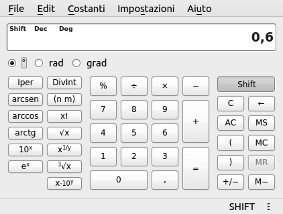
\includegraphics[scale=.55]{img/kcalc.png}
\end{inaccessibleblock}
 \caption{Calcolatrice KCalc.}\label{fig:G.4}
\end{minipage}
\end{figure}
\end{inaccessibleblock}

\emph{Dati}:~$\overline{AB}=5\unit{m}$\quad~$\overline{AH}=3\unit{m}$. 
\qquad\emph{Obiettivo}:~$\hat{\alpha}$.

\begin{soluzione}
 Partiamo dalla formula~$\overline{AH}=\overline{AB}\cdot \cos \alpha$, da essa 
possiamo ottenere
$\cos \alpha=\frac{\overline{AH}}{\overline{AB}}$. Sostituendo i valori noti 
otteniamo
$\cos \alpha=\frac{\overline{AH}}{\overline{AB}}=\frac{3}{5}=0,6$.

Per risalire dal valore del coseno al valore dell'angolo usiamo la calcolatrice 
attivando la funzione inversa di coseno; su molte calcolatrici
tale funzione è indicata con~$\cos^{-1}$, funzione che si attiva con il tasto 
\emph{Shift} (figura~\ref{fig:G.4}); nella calcolatrice
di esempio pigiando il tasto \emph{Shift} compare il tasto della funzione 
inversa \emph{arccos}.

Calcoliamo la misura dell'angolo il cui coseno è~$0,6$ immettendo tale valore e 
attivando i tasti \emph{Shift} e \emph{arccos}.
La calcolatrice restituisce~${\hat{\alpha}}= 53.13010235$.
Questo risultato ci dice che l'angolo è di~$53\grado$ più una parte 
decimale~$0.13010235$.
Ricordiamo che i sottomultipli del grado vengono espressi in sessantesimi ($1\, 
\text{grado}=60\, \text{primi}$),
a loro volta suddivisi in sessantesimi ($1\, \text{primo}=60\, \text{secondi}$).
Dunque la parte decimale estratta dalla calcolatrice va adeguatamente 
modificata:
al risultato della calcolatrice tolgo la parte intera~$(53)$ e moltiplico 
per~$60$ in questo caso ottengo~$7.8061\ldots$ la cui parte
intera rappresenta i primi; tolgo ancora la parte intera~$(7)$ e moltiplico 
per~$60$ ottenendo i secondi~$48.368\ldots$
Arrotondiamo la parte intera e possiamo 
concludere~$\hat{\alpha}{\approx}53\grado~7'48''$.
Alcune calcolatrici scientifiche fanno in automatico questi calcoli attivando un 
opportuno tasto.

Osserviamo che viene utilizzato il simbolo~${\approx}$ (uguale circa) per 
indicare che abbiamo usato valori approssimati.
Ora sei in grado di determinare l'ampiezza degli angoli acuti attivando le 
funzioni inverse sulla tua calcolatrice.
\end{soluzione}

% \ovalbox{\risolvii \ref{ese:G.3}, \ref{ese:G.4}, \ref{ese:G.5}}
% 
% \section{Operazioni con i gradi sessagesimali}
% \label{sec:trigo_gradisessagesimali}
% Accenniamo alle addizioni e sottrazioni tra angoli.
% 
% \begin{exrig}
%  \begin{esempio}
% Svolgiamo l'operazione~$48\grado~45' 52'' + 62\grado~27' 22''$.
% \begin{center}
%  % (c) 2012 Dimitrios Vrettos - d.vrettos@gmail.com

\begin{tikzpicture}[x=10mm,y=10mm]

\matrix (a) [matrix of nodes,matrix anchor=east] at (0,0){
48$\grado$&45'&52''&$+$\\
62$\grado$&27'&22''&{}\\
110$\grado$&72'&74''&{}\\
111$\grado$&13'&14''&{}\\};

\draw (a-2-1.south west) -- (a-2-4.south east);
\end{tikzpicture}
% \end{center}
% 
% 
% Sommando termine a termine otteniamo~$110\grado~72' 74''$. Tenendo conto che~1 
% grado equivale a~60 primi e~1 primo equivale a~60 secondi,
% si ha che i~$74\grado$ valgono~$1'$ e~$14''$, i~$72' 74''$ diventano 
% allora~$73'$ e~$14''$.
% Trasformiamo poi i~$73'$ in~$1\grado$ e~$13'$.
% 
% In definitiva si ha che~$110\grado~72' 74'' = 111\grado~13' 14''$.
%  \end{esempio}
% 
%  \begin{esempio}
% Svolgiamo ora una sottrazione:~$90\grado - 45\grado~33' 12''$.
% \begin{center}
%  % (c) 2012 Dimitrios Vrettos - d.vrettos@gmail.com

\begin{tikzpicture}[x=10mm,y=10mm]

\matrix (a) [matrix of nodes,matrix anchor=north] at (0,0){
90$\grado$&&&$-$\\
45$\grado$&33'&12''&{}\\};

\draw (a-2-1.south west) -- (a-2-3.south east);

\begin{scope}[xshift=14mm,yshift=-10mm,->, Maroon, thick]
\draw (0,0) -- (.5,0);
\end{scope}

\begin{scope}[xshift=35mm]
\matrix (a) [matrix of nodes,matrix anchor=north] at (0,0){
89$\grado$&59'&60''&$-$\\
45$\grado$&33'&12''&{}\\
44$\grado$&26'&48''&{}\\};

\draw (a-2-1.south west) -- (a-2-3.south east);
\end{scope}
\end{tikzpicture}
% \end{center}
% 
% Questa è una operazione molto comune, poiché capita abbastanza spesso di dover 
% calcolare l'angolo complementare.
% Per svolgere la sottrazione conviene scrivere~$90\grado$ come~$89\grado~59' 
% 60''$ e svolgere la sottrazione avendo come risultato~$44\grado~26' 48''$.
%  \end{esempio}
% 
%  \begin{esempio}
% Un'ultima sottrazione:~$72\grado~20' 40'' - 23\grado~40' 52''$.
% 
% Per fare questa sottrazione parto dai secondi e non potendo fare~40 - 52, 
% utilizzo il riporto trasformando in:~$72\grado~20' 40''$
% in~$72\grado~19' 100''$. Ora posso eseguire agevolmente la sottrazione e 
% ottengo~$48''$
% sottraggo poi i primi tra loro, aggiungendo il riporto ai~$19'$ e ottengo~$39'$ 
% sottraggo poi i gradi:~$71\grado - 23\grado$.
% Il risultato finale è~$48\grado~39' 48''$.
%  \end{esempio}
% \end{exrig}
% 
% \ovalbox{\risolvi \ref{ese:G.6}}

\section{Risoluzione di triangoli rettangoli}
\label{sec:trigo_triangolirettangoli}

Ricordiamo che risolvere un triangolo significa ricavare le misure di tutti i 
suoi elementi (lati e angoli) date le misure di alcuni dei suoi elementi.

\begin{exrig}
 \begin{esempio}
Determinate l'area del triangolo rettangolo sapendo che~${BC}=2\unit{m}$ 
e~$\hat{\beta} =20\grado$.

\emph{Dati}:~$\widehat{BAC}=90\grado$,\quad~$\overline{BC}=2\unit{m}$,
\quad~$\hat{\beta}=20\grado$.

\emph{Obiettivo}:~$\Area{(ABC)}$.

\emph{Procedura risolutiva}:
$\Area{(ABC)}=\frac{1}{2}\cdot \overline{AB}\cdot \overline{AC}$.

Dobbiamo dunque determinare le misure dei cateti. Applicando le definizioni:
\[\overline{AB}=\overline{BC}\cdot {\cos \beta}=2\cdot 
{\cos 20\grado} \approx2\cdot 0,9397\approx1,8794;\]
\[\overline{AC}=\overline{BC}\cdot {\cos \gamma}=2\cdot 
{\cos 70\grado} \approx2\cdot 0,3420\approx0,6840;\]
pertanto, $\Area\approx0.6428\unit{(m^{2})}$.
 \end{esempio}

 \begin{esempio}
Un triangolo rettangolo ha il cateto~$AB$ di~$5\unit{cm}$. e l'angolo acuto 
in~$C$ di~$57\grado$ determinate l'altro angolo acuto,
la misura del cateto~$AC$ e la misura dell'ipotenusa.

\emph{Dati}:~$\widehat{BAC}=90\grado$,\quad~$\widehat{BCA}=57\grado$,
\quad~$\overline{AB}=5\unit{cm}$.

\emph{Obiettivo}:~$\hat{\beta}$,\quad~$\overline{CA}$,\quad~$\overline{CB}$.

\emph{Procedura risolutiva}:
Essendo gli angoli acuti complementari si 
ottiene~$\hat{\beta}=90\grado-57\grado=33\grado$.
Per la formula inversa:
\[\overline{CB}=\frac{\overline{AB}}{\cos 
\beta}=\frac{5}{\cos 33\grado} \approx\frac{5}{0,8386}\approx5,9618\unit{cm}.\]
Infine determiniamo l'altro cateto e osserviamo che possiamo procedere in due 
modi:
\begin{itemize*}
 \item con il Teorema di Pitagora:
 
\[\overline{CA}=\sqrt{\overline{CB}^{2}-\overline{AB}^{2}}\approx\sqrt{35,
5432-25}\approx\sqrt{10,5432}\approx3,2470\unit{cm};\]
 \item per definizione:
 \[\overline{CA}=\overline{CB}\cdot \cos \gamma\approx5,9618 \cdot 
\cos 57\grado \approx5,9618\cdot 0,5446\approx3,2468\unit{cm}.\]
\end{itemize*}
\osservazione
\begin{enumeratea}
\item Nei calcoli effettuati abbiamo operato un'approssimazione; per esempio il 
valore esatto di~$\overline{CB}$ è rappresentato solo
dall'espressione~$\overline{CB}=\frac{\overline{AB}}{\cos 
\beta}=\frac{5}{\cos 33\grado}$.
\item I risultati ottenuti con procedimenti diversi possono differire, se pur di 
poco, a causa dell'uso di valori approssimati
nei calcoli che aumentano l'errore di approssimazione (propagazione 
dell'errore).
\end{enumeratea}
 \end{esempio}

 \begin{esempio}
Risolvi il triangolo rettangolo della figura sapendo che~$c=20\unit{cm}$ e~$\sin 
\beta=\frac{3}{5}$.
\begin{center}
 % (c) 2012 Dimitrios Vrettos - d.vrettos@gmail.com

\begin{tikzpicture}[x=9mm,y=9mm, font=\small]

  \coordinate (A) at (0,0);
  \coordinate (C) at ($(A)+(90:3)$);
  \coordinate (B) at ($(A)+(0:4)$);

  \draw (A) node[below left]{$A$}-- (C) node[above left]{$C$} -- (B)node[below right]{$B$} -- (A);

  \tkzMarkAngle[ fill=LimeGreen ,draw, size=.4](A,C,B)
  \tkzMarkAngle[ fill=LimeGreen ,draw, size=.4](C,B,A)
  \tkzMarkRightAngle[ fill=LimeGreen ,draw, size=.3](C,A,B)
  
  \begin{scope}[font=\scriptsize]
    \tkzLabelAngle[pos=.6](A,C,B){$\gamma$}
    \tkzLabelAngle[pos=.6](C,B,A){$\beta$}
    \tkzLabelAngle[pos=.6](C,A,B){$\alpha$}
  \end{scope}

  \tkzLabelSegment[midway, left](A,C){$b$}
  \tkzLabelSegment[midway, below](A,B){$c$}
  \tkzLabelSegment[midway, above](B,C){$a$}

  \begin{scope}[fill=CornflowerBlue, draw=black]
    \filldraw (0,0) circle (1pt);
    \filldraw (4,0) circle (1pt);
    \filldraw (0,3) circle (1pt);
  \end{scope}

\end{tikzpicture}
\end{center}
Usiamo l'identità fondamentale per determinare~$\cos \beta$:
\begin{align*}
&\cos \beta=\sqrt{1-\sin^{2} 
\beta}=\sqrt{1-\left(\frac{3}{5}\right)^{2}}=\sqrt{1-\frac{9}{25}}=
    \sqrt{\frac{25-9}{25}}=\sqrt{\frac{16}{25}}=\frac{4}{5};\\
&\cos \beta=\frac{c}{a}\Rightarrow a=\frac{c}{\cos \beta} = 
\frac{20}{\frac{4}{5}}=\frac{20\cdot{5}}{4}=25\unit{cm}.
\end{align*}

Per il teorema di 
Pitagora~$b=\sqrt{a^{2}-c^{2}}=\sqrt{25^{2}-20^{2}}=15\unit{cm}$
$\hat{\beta}\approx36\grado~52' 12''$ (calcolato con la calcolatrice e 
arrotondato), $\hat{\gamma}\approx90\grado - \hat{\beta} = 53\grado~07'48''$.
 \end{esempio}

 \begin{esempio}
Risolvere il triangolo rettangolo~$ABC$, retto in~$A$ (quello della figura 
precedente) sapendo che~$b=2\unit{cm}$ e~$\sin \beta=0,2$.

\emph{Dati}:~$b=2\unit{cm}$,\quad~$\sin \beta=0,2$.

\emph{Obiettivo}:~$a$,\quad~$c$,\quad~${\hat{\beta}}$,\quad~${\hat{\gamma}}$.

\emph{Procedura risolutiva}:
Dalle definizioni si ha
\[\sin \beta=\frac{b}{a} \Rightarrow~0,2=\frac{2}{a}\Rightarrow 
a=\frac{2}{0,2}=10\unit{cm}.\]
Con il teorema di Pitagora possiamo ricavare l'altro cateto
\[c=\sqrt{a^{2}-b^{2}}=\sqrt{100-4}=\sqrt{96}=4\sqrt{6}\approx9,7980\unit{cm}.\]
Infine con la funzione inversa ricaviamo 
l'angolo~${\hat{\beta}}$:~$\sin^{-1}(0,2)\approx11,5369\ldots$ e procedendo come 
spiegato in
precedenza otteniamo:~${\hat{\beta}}\approx11\grado~32' 13''$ e in 
seguito~${\hat{\gamma}}\approx90\grado-{\hat{\beta}}\approx78\grado~27'47''$.
 \end{esempio}
\end{exrig}

% \ovalbox{\risolvii \ref{ese:G.7}, \ref{ese:G.8}, \ref{ese:G.9}, \ref{ese:G.10}}

\subsection{Proiezione di un segmento lungo una direzione}

È dato un segmento~$AB$ ed una retta~$r$ che passa per un suo estremo ($A$, per 
fissare le idee). La
\emph{proiezione del segmento} $AB$ \emph{sulla retta} $r$ è il segmento~$AH$ 
dove~$H$ è l'intersezione fra~$r$ e la
perpendicolare alla retta~$r$ passante per~$B$ (si vedano i tre esempi in 
figura).
\begin{inaccessibleblock}[Una retta un segmento e 
la proiezione del segmento sulla retta.]
\begin{center}
 % (c) 2012 Dimitrios Vrettos - d.vrettos@gmail.com
% (c) 2020 Daniele Zambelli: daniele.zambelli@gmail.com

% \tkzLabelLine[⟨local options⟩](⟨pt1,pt2⟩){⟨label⟩}
% arguments
%  default
%  definition
% label
%  example \tkzLabelLine(A,B){δ}
% options
%  default
%  definition
% pos
%  .5
%  pos est une option de TikZ mais essentielle dans ce cas
% As an option, and in addition to the pos, you can use all styles of TikZ , especially the placement with above,
% right, ...

% \tkzDrawLine(A,B)
% \tkzLabelLine[pos=1.25,left](A,B){$(d_1)$}
% \

\begin{tikzpicture}[x=10mm,y=10mm, font=\small]

  \coordinate (A) at (0,0);
  \coordinate (H) at ($(A)+(0:3)$);
  \coordinate (B) at ($(H)+(90:2)$);

  \draw (B)node[above right]{$B$} -- (A) node[below]{$A$}-- (H) node[below]{$H$};
  \draw[dashed] (B)--(H);

  \draw (-.5,0) -- (3.5,0)node[below] {$r$};
  \tkzMarkAngle[ fill=LimeGreen ,draw, size=.4](H,A,B)

  \begin{scope}[font=\scriptsize]
    \tkzLabelAngle[pos=.6](H,A,B){$\alpha$}
  \end{scope}

  \begin{scope}[fill=CornflowerBlue, draw=black]
    \filldraw (0,0) circle (1pt);
    \filldraw (3,0) circle (1pt);
    \filldraw (3,2) circle (1pt);
  \end{scope}

  \begin{scope}[xshift=45mm]
    \tkzDefPoints{0/1/A, 2/0/B,1.25/1.59/H}
    \tkzDrawLine[add=0 and 0, dashed, thin](B,H)
    \tkzDrawLine[add=0 and 0,thin](A,B)
    \tkzMarkAngle[fill=LimeGreen ,draw, size=.4](B,A,H) 
%     \tkzDrawLine[add = .4 and .4, end=$r$, thin](A,H)
    \tkzDrawLine[add = .4 and .4, thin](A,H)
\tkzLabelLine[left](A,B){$r$}

    \tkzLabelPoint[above](H){$H$}
    \tkzLabelPoint[above](A){$A$}
    \tkzLabelPoint[below](B){$B$}
    
    \begin{scope}[font=\scriptsize]
      \tkzLabelAngle[pos=.6](H,A,B){$\alpha$}
    \end{scope}
    
    \tkzDrawPoints[fill=CornflowerBlue](A,B, H)
  \end{scope}

  \begin{scope}[xshift=80mm, rotate=-10]
    \tkzDefPoints{0/0/A, 0/2/H, 2/2/B}
    \tkzDrawLine[add=0 and 0, dashed, thin](B,H)
    \tkzDrawLine[add=0 and 0,thin](A,B)
%     \tkzDrawLine[add = 0 and .2, end=$r$, thin](A,H)
    \tkzDrawLine[add = 0 and .2, thin](A,H)

    \tkzLabelPoint[left](H){$H$}
    \tkzLabelPoint[below](A){$A$}
    \tkzLabelPoint[right](B){$B$}
    \tkzMarkAngle[fill=LimeGreen ,draw, size=.4](B,A,H) 

  \begin{scope}[font=\scriptsize]
    \tkzLabelAngle[pos=.6](H,A,B){$\alpha$}
  \end{scope}
    \tkzDrawPoints[fill=CornflowerBlue](A,B, H)
  \end{scope}
\end{tikzpicture}

\end{center}
\end{inaccessibleblock}

% \ovalbox{\risolvii \ref{ese:G.11}, \ref{ese:G.12}, \ref{ese:G.13}, 
% \ref{ese:G.14}, \ref{ese:G.15}, \ref{ese:G.16}, \ref{ese:G.17}, \ref{ese:G.18},
% \ref{ese:G.19}, \ref{ese:G.20}, \ref{ese:G.21}}

\section{Risoluzione di un triangolo qualsiasi con triangoli rettangoli}
\label{sec:trigo_altritriangoli}

Per risolvere i triangoli qualsiasi, tramite l'altezza, bisogna ricercare nella 
figura triangoli rettangoli.
Nel seguito saranno indicati altri teoremi che permettono
di risolvere tutti i tipi di triangoli.

\begin{exrig}
 \begin{esempio}
Risolvi il triangolo acutangolo della figura~\ref{fig:G.5} con~$\hat{\beta} 
=57\grado$, $\hat{\alpha} =39\grado$, $\overline{CH}=11\unit{m}$.
\begin{inaccessibleblock}[Figura: TODO]
 \begin{figure}[t]
\begin{minipage}[t]{.45\textwidth}
 \centering
 % (c) 2012 Dimitrios Vrettos - d.vrettos@gmail.com

\begin{tikzpicture}[x=10mm,y=10mm, font=\small]

  \coordinate (A) at (0,0);
  \coordinate (B) at ($(A)+(0:4.18)$);
  \coordinate (C) at ($(A)+(39:3.5)$);
  \coordinate (H) at ($(A)+(0:2.72)$);

  \draw (B) node[below right]{$B$}--(A) node[below left]{$A$}--(C) node[above]{$C$}--(B);

  \tkzMarkAngle[ fill=LimeGreen ,draw, size=.4](H,A,C)
  \tkzMarkAngle[ fill=LimeGreen ,draw, size=.4](A,C,B)
  \tkzMarkAngle[ fill=LimeGreen ,draw, size=.4](C,B,H)

  \draw (C)--(H) node[below]{$H$};

  \begin{scope}[font=\scriptsize]
    \tkzLabelAngle[pos=.6](H,A,C){$\alpha$}
    \tkzLabelAngle[left, pos=.6](A,C,B){$\gamma$}
    \tkzLabelAngle[pos=.6](C,B,H){$\beta$}
  \end{scope}
  
  \begin{scope}[fill=CornflowerBlue, draw=black]
    \filldraw (0,0) circle (1pt);
    \filldraw (4.18,0) circle (1pt);
    \filldraw (2.72,2.2) circle (1pt);
    \filldraw (2.72,0) circle (1pt);
  \end{scope}
\end{tikzpicture}
 \caption{Triangolo acutangolo.}\label{fig:G.5}
\end{minipage}\hfil
\begin{minipage}[t]{.45\textwidth}
\centering
 % (c) 2012 Dimitrios Vrettos - d.vrettos@gmail.com

\begin{tikzpicture}[x=10mm,y=10mm, font=\small]

  \coordinate (A) at (0,0);
  \coordinate (B) at ($(A)+(0:4.26)$);
  \coordinate (C) at ($(B)+(145:3.486)$);
  \coordinate (D) at ($(A)+(90:2)$);

  \draw (D) node[above left]{$D$}--(A) node[below left]{$A$}--(B) node[below right]{$B$}--(C)node [above right]{$C$} --(D);

  \tkzMarkAngle[ fill=LimeGreen ,draw, size=.4](C,A,D)
  \tkzMarkAngle[ fill=LimeGreen ,draw, size=.4](A,C,B)
  \tkzMarkAngle[ fill=LimeGreen ,draw, size=.4](C,B,A)

  \draw[dashed] (C)--(A);

  \begin{scope}[fill=CornflowerBlue, draw=black]
    \filldraw (0,0) circle (1pt);
    \filldraw (4.26,0) circle (1pt);
    \filldraw (1.4,2) circle (1pt);
    \filldraw (0,2) circle (1pt);
  \end{scope}
\end{tikzpicture}
\caption{Trapezio rettangolo.}\label{fig:G.6}
\end{minipage}
 \end{figure}
\end{inaccessibleblock}

Ricordando che la somma degli angoli di un triangolo è~$180\grado$ 
ricaviamo~$\hat{\gamma}$:
\[ \hat{\gamma} =180\grado-\hat{\alpha} -\hat{\beta} 
=180\grado-39\grado-57\grado=84\grado.\]
Individuiamo ora i triangoli rettangoli nella figura in modo da poter applicare 
le formule.

Con il triangolo rettangolo~$CHB$:
\begin{align*}
 &\sin \beta=\frac{\overline{CH}}{\overline{CB}} \Rightarrow 
\overline{CB}=\frac{\overline{CH}}{\sin \beta}=
    \frac{11}{\sin 57\grado}\approx13,2\unit{m};\\
&\tan \beta=\frac{\overline{CH}}{\overline{BH}} \Rightarrow 
\overline{BH}=\frac{\overline{CH}}{\tan \beta}=
    \frac{11}{\tan(57\grado)}\approx7,15\unit{m}.
\end{align*}

Con il triangolo rettangolo~$AHC$:
\begin{align*}
&\sin (\alpha )=\frac{\overline{CH}}{\overline{AC}} \Rightarrow 
\overline{AC}=\frac{\overline{CH}}{\sin \alpha}=
    \frac{11}{\sin 39\grado}\approx17,46\unit{m};\\
&\tan \alpha=\frac{\overline{CH}}{\overline{AH}} \Rightarrow 
\overline{AH}=\frac{\overline{CH}}{\tan \beta}=
    \frac{11}{\tan(39\grado)}\approx13,75\unit{m}.
\end{align*}

Infine 
calcolo~$\overline{AB}=\overline{AH}+\overline{BH}\approx7,15+13,75\approx20,
9\unit{m}$.
 \end{esempio}
\end{exrig}

% \ovalbox{\risolvii \ref{ese:G.22}, \ref{ese:G.23}, \ref{ese:G.24}, 
% \ref{ese:G.25}}

\subsection{Quadrilateri}
\label{subsec:trigo_quadrilatei}

\begin{exrig}\vspace{1.10ex}
 \begin{esempio}
Nel trapezio rettangolo~$ABCD$ (figura~\ref{fig:G.6}) il lato obliquo~$BC$ forma 
un angolo di~$35\grado$ con la base maggiore~$AB$, inoltre la diagonale~$AC$
è perpendicolare a~$BC$. Calcola il perimetro e l'area del trapezio sapendo che 
la sua altezza è~$10\unit{cm}$.

Ricordando che la somma degli angoli di un triangolo è~$180\grado$ 
ricaviamo~$\widehat{CAB}=55\grado$.
Siccome il trapezio è rettangolo
$\widehat{DAC}=\widehat{DAB}-\widehat{CAB}=90\grado-55\grado$.
Calcoliamo ora~$CB$, $AB$ e~$DC$:
\begin{align*}
&\sin \widehat{ABC} =\frac{\overline{AD}}{\overline{CB}} \Rightarrow 
\overline{CB}=\frac{\overline{AD}}{\sin \widehat{ABC}}=\frac{10}{\sin 35\grado
}\approx17,43\unit{cm};\\
&\overline{AB}=\frac{\overline{CB}}{\cos \widehat{ABC}}\approx\frac{17,43}{
\cos 55\grado}\approx21,28\unit{cm};\\
&\frac{\overline{DC}}{\overline{AD}}=\tan(\widehat{DAC}) \Rightarrow 
\overline{DC}=\overline{AD}\cdot\tan(\widehat{DAC})=10\tan(35\grado)\approx7,00.
\end{align*}


Da cui:
\begin{align*}
&2p=\overline{AB}+\overline{BC}+\overline{DC}+\overline{DA}\approx21,28+17,43+7,
00+10\approx55,71\unit{cm};\\
&\Area=\frac{(\overline{AB}+\overline{DC})\cdot\overline{AD}}{2}\approx\frac{(21
,28+7,00)\cdot 10}{2}\approx~141,40\unit{cm^2}.
\end{align*}
 \end{esempio}
\end{exrig}

% \ovalbox{\risolvii \ref{ese:G.26}, \ref{ese:G.27}, \ref{ese:G.28}, 
% \ref{ese:G.29},\ref{ese:G.30}, \ref{ese:G.31}, \ref{ese:G.32}, \ref{ese:G.33}}

\subsection{Applicazioni della trigonometria}
\label{subsec:trigo_applicazioni}

La topografia è una disciplina che studia gli strumenti ed i metodi operativi, 
sia di calcolo sia di disegno, che sono necessari per ottenere
una rappresentazione grafica di una parte della superficie terrestre.
La topografia ha carattere applicativo e trae la sua base teorica dalla 
matematica, dalla geometria e dalla trigonometria.

\begin{exrig}
 \begin{esempio}
Risolvere il quadrilatero della figura\ref{fig:G.7} sapendo 
che~$AB=42,5\unit{m}$, $BC=32,18\unit{m}$, $CD=27,6\unit{m}$,
$\widehat{BAD}=56\grado$, $\widehat{ADC}=62\grado$.
\begin{inaccessibleblock}[Figura: TODO]
 \begin{figure}[t]
\centering
% (c) 2012 Dimitrios Vrettos - d.vrettos@gmail.com

\begin{tikzpicture}[x=10mm,y=10mm, font=\small]

\coordinate (A) at (0,0);
\coordinate (D) at ($(A)+(0:6.702)$);
\coordinate (B) at ($(A)+(56:4.25)$);
\coordinate (C) at ($(D)+(118:2.76)$);
\coordinate (F) at ($(A)+(0:2.38)$);
\coordinate (G) at ($(F)+(90:2.43)$);
\coordinate (E) at ($(A)+(0:5.4)$);

\draw (B) node[above]{$B$}--(A) node[below left]{$A$}--(D) node[below right]{$D$}--(C)node [right]{$C$} --(B);

\tkzMarkAngle[ fill=LimeGreen ,draw, size=.4](D,A,B)
\tkzMarkAngle[ fill=LimeGreen ,draw, size=.4](C,D,A)

\begin{scope}[dashed]
\draw(B)--(F) node[below]{$F$};
\draw(C)--(G)node[left]{$G$};
\draw(C)--(E)node[below]{$E$};
\end{scope}

\begin{scope}[fill=CornflowerBlue, draw=black]
\filldraw (0,0) circle (1pt);
\filldraw (6.702,0) circle (1pt);
\filldraw (5.4,2.43) circle (1pt);
\filldraw (2.38,3.52) circle (1pt);
\filldraw (2.38,0) circle (1pt);
\filldraw (2.38,2.43) circle (1pt);
\filldraw (5.4,0) circle (1pt);
\end{scope}
\end{tikzpicture}
\caption{Il quadrilatero~$ABCD$.}\label{fig:G.7}
\end{figure}
\end{inaccessibleblock}

\emph{Dati}:~$\overline{AB}=42,5\unit{m}$,\quad~$\overline{BC}=32,18\unit{m}$,
\quad~$\overline{CD}=27,6\unit{m}$,\quad~$\widehat{BAD}=56\grado$,
\quad~$\widehat{ADC}=62\grado$.

\emph{Obiettivo}:~$\overline{AD}$,\quad~$\widehat{ABC}$,\quad~$\widehat{CDA}$.

\emph{Procedura risolutiva}:
Suddividiamo il quadrilatero in tre triangoli rettangoli e in un rettangolo, 
come nella figura riportata sotto e risolviamo i triangoli.

Triangolo~$FBA$:
\begin{align*}
&\widehat{FBA}=90\grado-\widehat{BAD}=90\grado-56\grado=34\grado;\\
&\overline{AF}=\overline{AB}\cos \widehat{BAD} = 42,5\cos 56\grado \approx23,
77\unit{m};\\
&\overline{BF}=\overline{AB}\sin \widehat{BAD} =42,5 \sin 56\grado\approx35,
23\unit{m}.
\end{align*}

Triangolo~$DCE$:
\begin{align*}
 &\widehat{DCE}=90\grado-\widehat{ADC}=90\grado-62\grado=28\grado;\\
&\overline{DE}=\overline{CD}\cos \widehat{FBA}=27,6\cos 62\grado \approx12,
96\unit{m};\\
&\overline{CE}=\overline{CD}\sin \widehat{ADC} =27,6 \sin 62\grado \approx24,
37\unit{m}.
\end{align*}

Triangolo~$GBC$:
\begin{align*}
&\overline{BG}=\overline{BF}-\overline{GF}=\overline{BF}-\overline{CE}\approx35,
23-24,37\approx10,86\unit{m};\\
&\cos \widehat{CBG}=\frac{\overline{GB}}{\overline{CB}}=\frac{10,86}{32,18}
\approx0,34\Rightarrow\cos^-1(0,34)\approx70\grado~16' 36'';\\
&\widehat{BCG}=90\grado-\widehat{CBG}\approx90\grado-70\grado~16' 
36''\approx19\grado~43' 24'';\\
&\overline{GC}=\overline{BC}\sin (70\grado~16' 36'')=30,29\unit{m}.
\end{align*}

Calcoliamo ora gli elementi incogniti del quadrilatero:
\begin{align*}
&\overline{DA}=\overline{AF}+\overline{FE}+\overline{ED}\approx23,77+30,29+12,
96\approx67,02\unit{m};\\
&\widehat{ABC}=\widehat{ABF}+\widehat{FBC}\approx34\grado+70\grado~16' 
36''\approx104\grado~16' 36'';\\
&\widehat{BCD}= \widehat{BCG}+\widehat{GCE}+\widehat{ECD}\approx19\grado~43' 
24''+90\grado+34\grado\approx143\grado~43' 24''.
\end{align*}
\end{esempio}
\end{exrig}

% \ovalbox{\risolvii \ref{ese:G.34}, \ref{ese:G.35}, \ref{ese:G.36}, 
% \ref{ese:G.37}, \ref{ese:G.38}, \ref{ese:G.39}, \ref{ese:G.40}, \ref{ese:G.41}, 
% \ref{ese:G.42}}
% 
% \vspazio\ovalbox{\ref{ese:G.43}, \ref{ese:G.44}, \ref{ese:G.45}, \ref{ese:G.46}}

\section{Risoluzione di un triangolo qualunque}
\label{sec:trigo_triangoloqualunque}

Le funzioni trigonometriche possono essere calcolate anche su angoli maggiori 
di~$90\grado$. Poiché, al momento, siamo interessati alle
applicazioni sui triangoli, ci basterà estendere le nostre considerazioni agli 
angoli compresi fra~$90\grado$ e~$180\grado$,
essendo~$180\grado$ la misura limite superiore di un angolo interno di un 
triangolo.
\begin{exrig}
 \begin{esempio}
Analizziamo la tabella con i valori approssimati alla quarta cifra decimale 
delle funzioni seno e coseno per alcuni angoli da~$0\grado$ a~$180\grado$.
\[
\begin{array}{cccccccccccc}
\toprule
\text{angolo}&0\grado &30\grado &45\grado &60\grado &90\grado & 120\grado & 
135\grado &150\grado &180\grado\\
\midrule
\sin \alpha& 0 & 0,5 & 0,7071 & 0,8660 & 1 & 0,8660 & 0,7071 & 0,5 & 0\\
\cos \alpha& 1 & 0,8660 & 0,7071 & 0,5 & 0 & -0,5 & -0,7071 & -0,8660 &-1\\
\bottomrule
\end{array}
\]
Dalla tabella si nota che la funzione seno si mantiene positiva nell'intervallo 
($0\grado$ $180\grado$), nei cui estremi si annulla.
Inoltre essa assume il valore massimo, uguale a~1, quando l'angolo è 
di~$90\grado$.
La funzione coseno, invece, è negativa per angoli compresi tra~$90\grado$ 
e~$180\grado$. Precisamente: essa decresce da~$1$ a~$0$
man mano che l'angolo su cui è calcolata cresce da~$0\grado$ a~$90\grado$, 
dopodiché continua a decrescere, da~$0$ a~$-1$,
man mano che l'angolo passa da~$90\grado$ a~$180\grado$, si annulla~$90\grado$.
Osserviamo anche che angoli supplementari hanno lo stesso seno e coseno opposto.
Queste considerazioni saranno chiarite con lo studio delle funzioni circolari.
 \end{esempio}
\end{exrig}
Affrontiamo ora il problema di risolvere un triangolo qualsiasi.
Come sappiamo, gli elementi caratteristici di un triangolo sono le misure dei 
suoi lati e dei suoi angoli.
Sappiamo anche che per determinare univocamente un triangolo sono, in linea di 
massima, necessari solo tre di questi elementi
purché uno almeno di questi sia un lato. Ciò deriva dai tre criteri di 
congruenza dei triangoli che andiamo a ricordare.

\paragraph{Primo criterio di congruenza} Due triangoli che abbiano 
rispettivamente congruenti due lati e l'angolo tra essi
compreso sono congruenti.

\paragraph{Secondo criterio di congruenza}
Due triangoli che abbiano rispettivamente congruenti un lato e due
angoli ugualmente posti rispetto al lato sono congruenti.

\paragraph{Terzo criterio di congruenza}
Due triangoli che abbiano rispettivamente congruenti i tre lati sono congruenti.

Ricordiamo che due triangoli che abbiano ordinatamente uguali tutti gli angoli 
non sono, in generale, congruenti, bensì sono \emph{simili}.

Quello che ci chiediamo è se la trigonometria, finora usata solo per i triangoli 
rettangoli, ci possa venire in aiuto per la
determinazione delle misure degli elementi incogniti di un triangolo qualunque, 
quando conosciamo i tre elementi che lo
determinano univocamente. Ad esempio, se è assegnata la lunghezza di due lati e 
l'ampiezza dell'angolo compreso,
la geometria euclidea, ci aiuta a costruire il suddetto triangolo tramite riga e 
compasso ma non ci dice nulla delle
misure degli elementi incogniti.

Disegniamo un triangolo avendo cura di indicare con la stessa lettera vertice e 
lato opposto e di nominare con
${\hat{\alpha}}$, ${\hat{\beta}}$, ${\hat{\gamma}}$ le ampiezze degli angoli di 
vertice rispettivamente~$A$, $B$, $C$.
\begin{center}
 % (c) 2012 Dimitrios Vrettos - d.vrettos@gmail.com

\begin{tikzpicture}[x=10mm,y=10mm, font=\small]

\coordinate (A) at (0,0);
\coordinate (B) at ($(A)+(40:4)$);
\coordinate (C) at ($(A)+(0:2.5)$);

\draw (A) node[below left]{$A$}--(B) node[above]{$B$}--(C)node [below right]{$C$} --(A);

\tkzMarkAngle[ fill=LimeGreen ,draw, size=.4](C,A,B)
\tkzMarkAngle[ fill=LimeGreen ,draw, size=.4](A,B,C)
\tkzMarkAngle[ fill=LimeGreen ,draw, size=.4](B,C,A)

\tkzLabelSegment[midway, below](A,C){$b$}
\tkzLabelSegment[midway, above](A,B){$c$}
\tkzLabelSegment[midway, right](B,C){$a$}

\begin{scope}[font=\scriptsize]
\tkzLabelAngle[pos=.6](C,A,B){$\alpha$}
\tkzLabelAngle[pos=.6](A,B,C){$\beta$}
\tkzLabelAngle[pos=.6](B,C,A){$\gamma$}
\end{scope}

\begin{scope}[fill=CornflowerBlue, draw=black]
\filldraw (0,0) circle (1pt);
\filldraw (2.5,0) circle (1pt);
\filldraw (3.05,2.55) circle (1pt);
\end{scope}
\end{tikzpicture}
\end{center}


\subsection{Caso I: due lati e l'angolo compreso congruenti}

Come abbiamo premesso, assegnati due lati e l'angolo tra essi compreso, la 
geometria euclidea ci assicura l'esistenza
di un solo triangolo che soddisfi i dati, ma non ci permette di determinare la 
misura del terzo lato, né le ampiezze degli altri angoli.
Per questo ci viene in aiuto il seguente

\begin{teorema}[del coseno o di Carnot]
In un triangolo qualsiasi di cui siano note le lunghezze di due lati e 
l'ampiezza dell'angolo compreso, il quadrato della lunghezza
del lato incognito è uguale alla somma dei quadrati delle lunghezze note 
diminuita del loro doppio prodotto per il coseno dell'angolo compreso.
A seconda di quali siano i due lati noti, traducendo in linguaggio matematico 
quanto afferma l'enunciato si ha:
\begin{align*}
&c^{2}=a^{2}+b^{2}-2\cdot a\cdot b\cdot \cos \gamma;\\
&a^{2}=c^{2}+b^{2}-2\cdot c\cdot b\cdot \cos \alpha;\\
&b^{2}=a^{2}+c^{2}-2\cdot a\cdot c\cdot \cos  \beta.
\end{align*}
\end{teorema}

\begin{problema}
Risolvete il triangolo~$ABC$ dati~$a= 20\unit{cm}$, $b=10\unit{cm}$, 
${\hat{\gamma}}=36\grado$.
\end{problema}

\emph{Dati}:~$a= 
20\unit{cm}$,\quad~$b=10\unit{cm}$,\quad~${\hat{\gamma}}=36\grado$.

\emph{Obiettivo}:~$c$,\quad~$\hat{\alpha}$,\quad~$\hat{\beta}$.

\emph{Procedura risolutiva}:
per il teorema di Carnot possiamo scrivere
\begin{align*}
&c^{2}=a^{2}+b^{2}-2\cdot a\cdot b\cdot \cos  \gamma\\
\Rightarrow &c^{2}=20^{2}+10^{2}-2\cdot 20\cdot 10\cdot 
\cos 36\grado \approx400+100-400\cdot 0,8090\approx176,4\\
\Rightarrow &c\approx\sqrt{176,4}\approx13,2815\unit{cm}.
\end{align*}

Ora dobbiamo determinare gli altri due angoli; utilizzando ancora il teorema di 
Carnot nella formula
$a^{2}=c^{2}+b^{2}-2\cdot c\cdot b\cdot \cos  \alpha$ 
conoscendo i tre lati ci rimane come incognita il cos(${\alpha}$). 
Sostituiamo i valori noti:~$20^{2}=176,4+10^{2}-2\cdot 
13,2815\cdot 10\cdot \cos  \alpha$, eseguiamo i calcoli
$400\approx~276,4-265,63\cdot \cos  \alpha$ e da questa ricaviamo~$\cos  
\alpha\approx \frac{276,4-400}{265,63}\approx-0,4653$ da cui
$\hat{\alpha}\approx\cos ^{-1}(-0,4653)\approx~117\grado$. Il triangolo è 
ottusangolo i suoi lati misurano rispettivamente
$a=20\unit{cm}$, $b=10\unit{cm}$, $c=13.2815\unit{cm}$ i suoi angoli hanno 
ampiezza~$\hat{\alpha} =117\grado$, $\hat{\beta} =36\grado$, $\hat{\gamma} 
=27\grado$.

\subsection{Caso II: tre lati congruenti}
Sappiamo dalla geometria euclidea che assegnati tre segmenti affinché si possa 
costruire il triangolo che li ha come lati
deve essere verificato il teorema della disuguaglianza triangolare: ``in ogni 
triangolo ogni lato deve essere minore della somma
degli altri due e maggiore della loro differenza''.

\begin{problema}
Determinate le ampiezze degli angoli di un triangolo note le misure dei suoi 
lati~$a=5\unit{m}$, $b=12\unit{m}$, $c=13\unit{m}$.
\end{problema}

\emph{Dati}:~$a= 5\unit{m}$,\quad~$b=12\unit{m}$,\quad~$c=13\unit{m}$.

\emph{Obiettivo}:~$\hat{\alpha}$,\quad~$\hat{\beta}$,\quad~$\hat{\gamma}$.

\emph{Procedura risolutiva}:
utilizziamo almeno due volte il teorema del coseno per determinare due angoli. 
Per trovare~$\cos \gamma$ utilizziamo
$c^{2}=a^{2}+b^{2}-2\cdot a\cdot b\cdot \cos \gamma$, sostituendo i dati si 
ottiene~$13^{2}=5^{2}+12^{2}-2\cdot 5\cdot 12\cdot \cos \gamma$,
da cui~$\cos \gamma=\frac{25+144-169}{120}=0$.
Per trovare~$\cos \alpha$ utilizziamo ancora il teorema di Carnot nella formula
$a^{2}=c^{2}+b^{2}-2\cdot c\cdot b\cdot \cos \alpha$. Sostituiamo i valori 
noti:~$25=169+144-312\cdot \cos \alpha$,
da cui~$\cos \alpha=\frac{169+144-25}{312}=0,9230$.
Quindi~$\hat{\gamma}=\cos^{-1}(0)=90\grado$, 
$\hat{\alpha}\approx\cos^{-1}(0,9230)\approx22\grado$, 
$\hat{\beta}=180\grado-90\grado-22\grado=68\grado$.

\subsection{Caso III: un lato e gli angoli congruenti}
Se conosciamo solo un lato, e due angoli, ci serve il seguente

\begin{teorema}[dei seni o di Euler]
In un triangolo qualsiasi risulta costante il rapporto fra la lunghezza di un 
lato e il seno dell'angolo che gli è opposto. In formule:
\[\frac{a}{\sin \alpha}=\frac{b}{\sin \beta}=\frac{c}{\sin \gamma}.\]
\end{teorema}

\begin{problema}
Risolvete il triangolo~$ABC$ sapendo che~$a= 7,52\unit{m}$, 
$\hat{\beta}=98\grado$, ${\hat{\gamma}}=27\grado$.
\end{problema}

\emph{Dati}:~$a= 
7,52\unit{m}$,\quad~$\hat{\beta}=98\grado$,\quad~${\hat{\gamma}}=27\grado$.

\emph{Obiettivo}:~$b$,\quad~$c$,\quad~$\hat{\alpha}$.

\emph{Procedura risolutiva}:
Possiamo immediatamente determinare il terzo angolo: 
\[{\hat{\alpha}}=180\grado-(98\grado+27\grado)=55\grado.\]
Per determinare i lati~$b$ e~$c$ applichiamo il teorema di Euler.

Per la prima uguaglianza del teorema otteniamo:
\[
\frac{7,52}{\sin 55\grado}=\frac{b}{\sin 98\grado} \Rightarrow 
b=\frac{7,52}{\sin 55\grado}\cdot \sin 98\grado\approx
\frac{7,52}{0,8192}\cdot 0,9902\approx~9,0897\unit{m}.
\]
Considerando l'uguaglianza tra il primo e l'ultimo rapporto del teorema 
otteniamo:
\[
\frac{7,52}{\sin 55\grado}=\frac{c}{\sin 27\grado} \Rightarrow 
c=\frac{7,52}{\sin 55\grado}\cdot \sin 27\grado\approx~4,1674\unit{m}.
\]
\subsection{Riflessioni sull'uso del teorema dei seni}
\begin{problema}
Risolvete il triangolo~$ABC$ sapendo che~$a= 20\unit{cm}$, $c= 13\unit{cm}$, 
${\hat{\gamma}}=36\grado$.
\end{problema}

\emph{Dati}:~$a= 20\unit{cm}$,\quad~$c= 
13\unit{cm}$,\quad~${\hat{\gamma}}=36\grado$.

\emph{Obiettivo}:~$b$,\quad~$\hat{\alpha}$,\quad~$\hat{\beta}$.

Gli elementi noti non rispecchiano le condizioni sufficienti di alcuno dei 
criteri di congruenza, ma possiamo usare il teorema dei seni
che ci assicura che in qualunque triangolo si ha
 \[\frac{a}{\sin \alpha}=\frac{b}{\sin \beta}=\frac{c}{\sin \gamma}\]
e quindi
\[\frac{20}{\sin \alpha}=\frac{13}{\sin 36\grado}\Rightarrow\sin 
\alpha=\frac{20\cdot\sin 36\grado}{13}\approx~0,9043,\]
e dunque con la funzione inversa~$\sin^{-1}(0,9043)$ possiamo ricavare 
l'angolo~${\hat{\alpha}}\approx~64\grado$ e 
dunque~${\hat{\beta}}{\approx}80\grado$.

Sembrerebbe tutto corretto, ma abbiamo trascurato il fatto che angoli 
supplementari hanno lo stesso seno dunque
da~$\sin ^{-1}(0,9043)$ si può ottenere~${\hat{\alpha}}{\approx} 64\grado$ 
oppure~${\hat{\alpha}}{\approx}116\grado$,
e dunque il triangolo non è univocamente determinato. Proseguendo nel 
ragionamento avremmo:
\paragraph{Caso I}
${\hat{\alpha}}{\approx}64\grado$, quindi il triangolo è acutangolo 
e~${\hat{\beta}}{\approx} 80\grado$ possiamo determinare~$b$ applicando 
nuovamente
il teorema dei seni
\[\frac{13}{\sin 36\grado}=\frac{b}{\sin 80\grado}\Rightarrow 
b=\frac{13\cdot0,9848}{0,5877}\approx21\unit{cm}.\]
\paragraph{Caso II}
${\hat{\alpha}}{\approx}116\grado$, quindi il triangolo è ottusangolo 
e~${\hat{\beta}}{\approx} 28\grado$ possiamo determinare~$b$ con
il teorema dei seni
\[\frac{13}{\sin 36\grado}=\frac{b}{\sin 28\grado}\Rightarrow 
b=\frac{13\cdot0,4694}{0,5877}\approx10\unit{cm}.\]

Il problema ha due soluzioni.
\begin{problema}
Risolvete il triangolo~$ABC$ sapendo che~$a= 26\unit{m}$, $b= 12\unit{m}$, 
${\hat{\alpha}}=124\grado$.
\end{problema}

\emph{Dati}:~$a= 26\unit{m}$,\quad~$b= 
12\unit{m}$,\quad~${\hat{\alpha}}=124\grado$.

\emph{Obiettivo}:~$c$,\quad~$\hat{\beta}$,\quad~$\hat{\gamma}$.

Applichiamo il teorema dei seni:
\[\frac{13}{\sin 124\grado}=\frac{12}{\sin \beta}\Rightarrow \sin 
\beta=\frac{12\cdot\sin 124\grado}{26}\approx\ldots \ldots \ldots.\]
In questo caso non ci sono dubbi: un triangolo non può avere due angoli ottusi. 
Potete completare voi la soluzione e otterrete
${\beta}{\approx}\ldots\ldots$ quindi~${\hat{\gamma}}{\approx} \ldots\ldots$ e 
infine~$c{\approx}\ldots\ldots$

\begin{problema}
Risolvete il triangolo~$ABC$ sapendo che~$a= 9\unit{m}$, $b=2 \sqrt 3\unit{m}$, 
${\hat{\beta}}=30\grado$.
\end{problema}
Come nel caso precedente abbiamo la misura di due lati e l'angolo opposto ad uno 
di essi; dunque per il teorema dei seni si ha
\[\frac{a}{\sin \alpha}=\frac{b}{\sin \beta} \Rightarrow \frac{9}{\sin 
\alpha}=\frac{2\sqrt{3}}{\sin 30\grado} \Rightarrow \frac{9}{\sin 
\alpha}=\frac{2\sqrt{3}}{0,5},\]
da cui~$\sin  \alpha=1,29$, impossibile! Il seno di un angolo ha come valore 
massimo~1.
Il problema non ha alcuna soluzione.

% \vspazio\ovalbox{\risolvii \ref{ese:G.68}, \ref{ese:G.69}, \ref{ese:G.70}, 
% \ref{ese:G.71}, \ref{ese:G.72}, \ref{ese:G.73}, \ref{ese:G.74}}
